\setlength{\parindent}{0em}
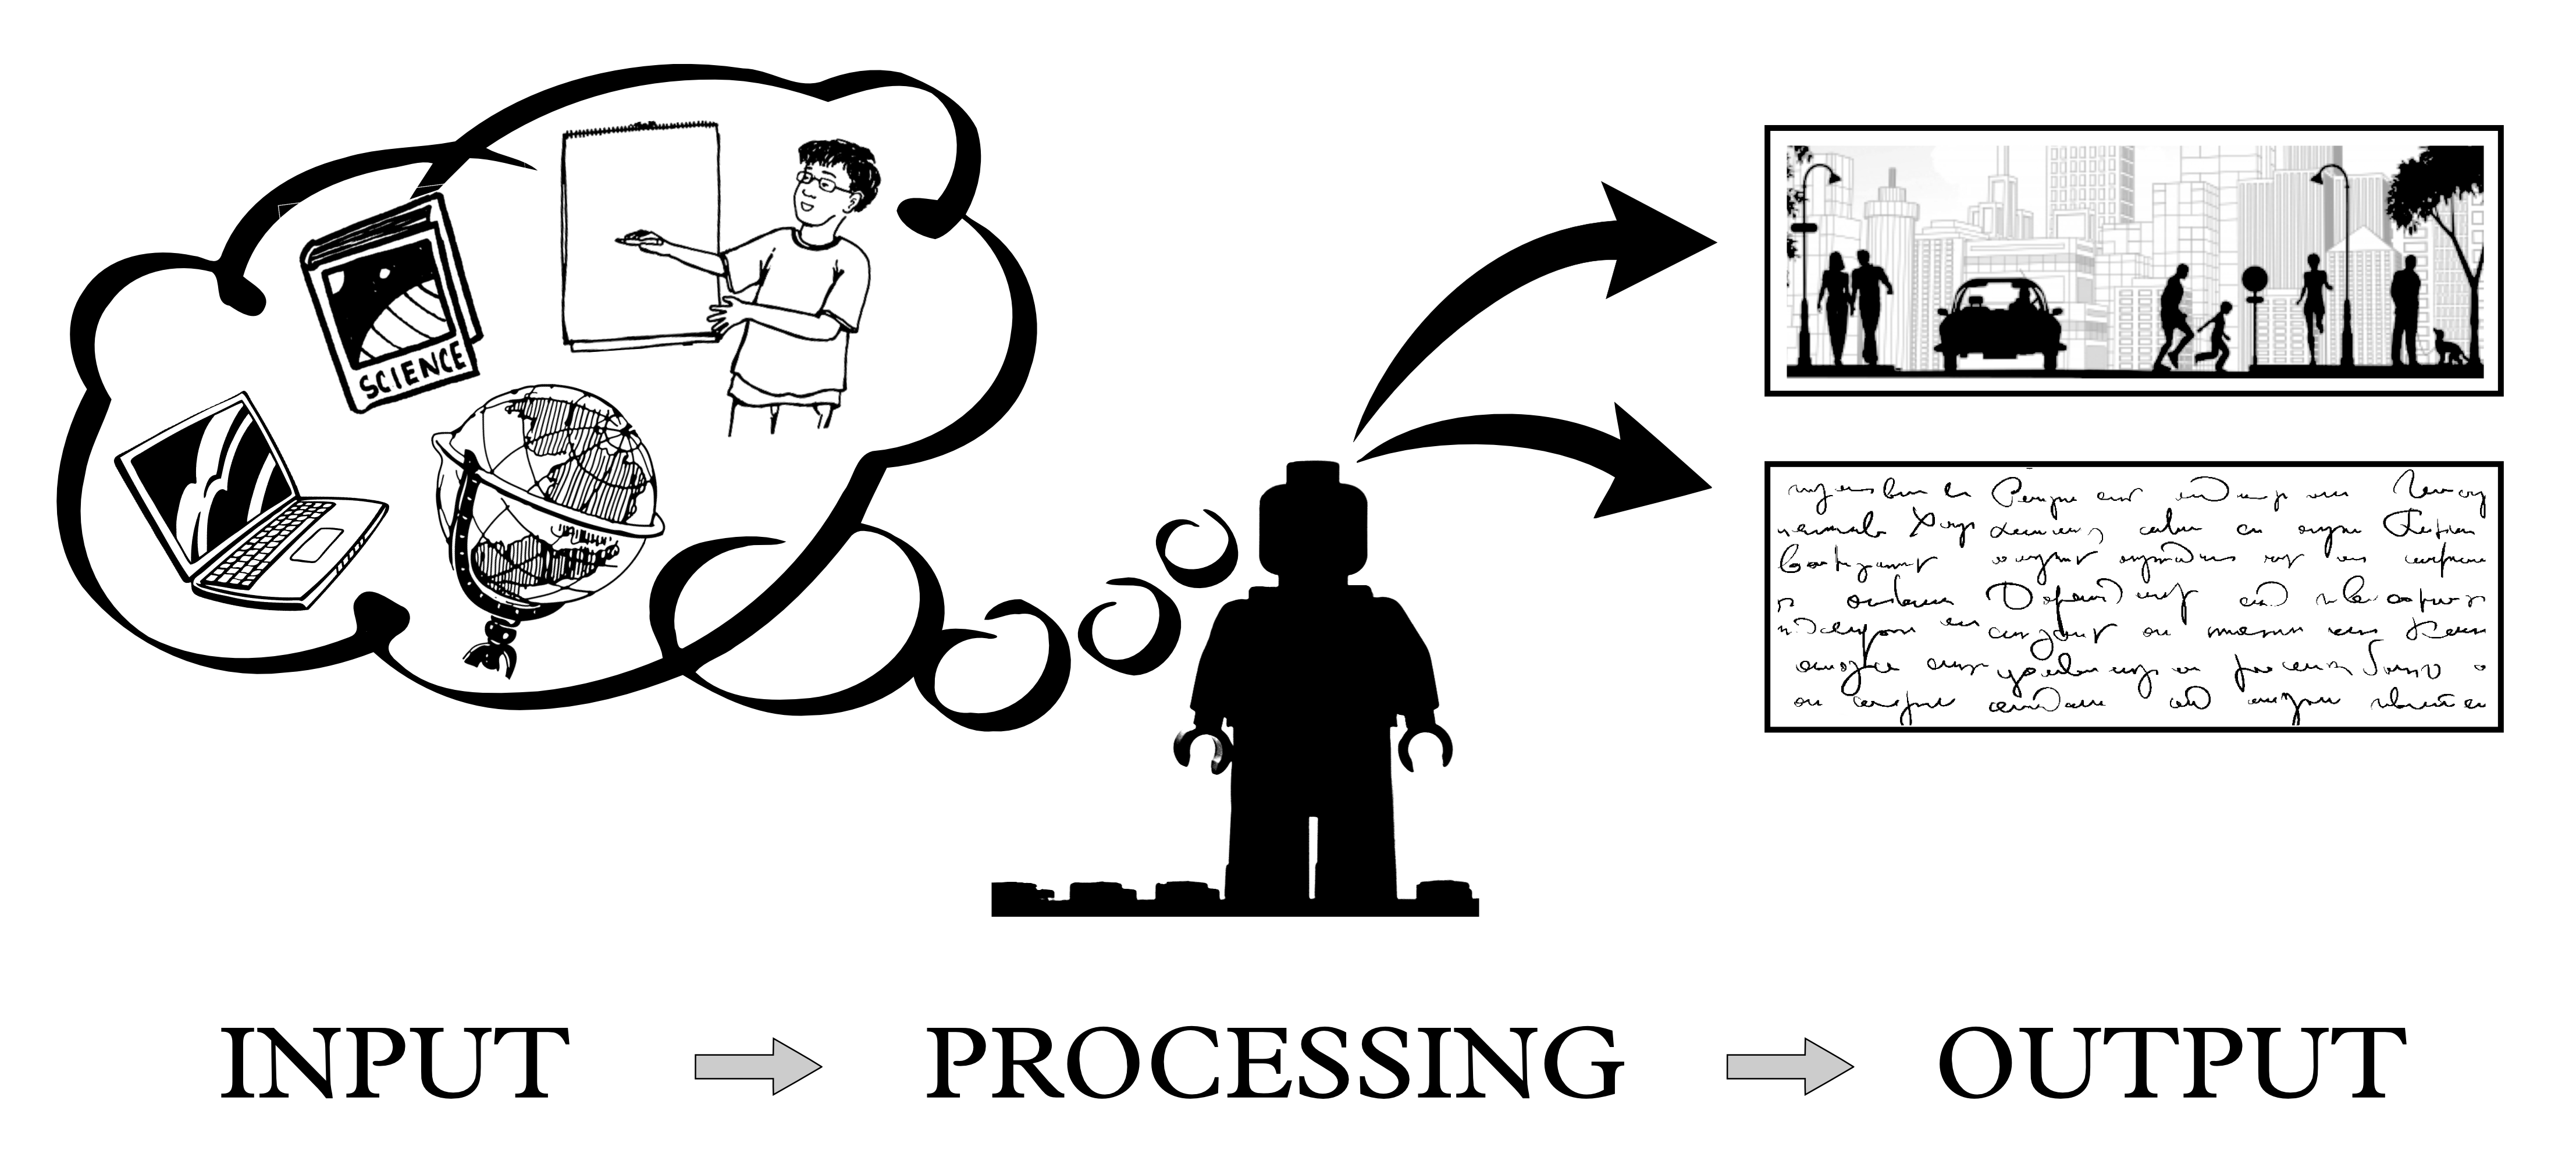
\includegraphics[width=\textwidth]{../../../img/innersim.png}

When you move to catch a falling pen, or notice that your friend is upset just by the way they entered the room, you're using your \textbf{inner simulator}.
\begin{center}
	\begin{tabular}{ | p{.5\textwidth} | p{.5\textwidth} | }
		\hline
		\textbf{Inner Simulator} & \textbf{Explicit/Verbal Models} \\ \hline
		Intuitive; part of System 1 & Analytical; part of System 2 \\ \hline
		Outputs feelings, urges, reflexes, and vivid predictions (sometimes called ``anticipations'') & Outputs arguments, calculations, and explicit models (sometimes called ``professions'') \\ \hline
		Learns well from experience and examples and responds to being \emph{shown} & Learns well from textbooks, statistics, Wikipedia, etc. and responds to being \emph{told} \\ \hline
		Good at social judgment, routine tasks, and any situation where you have lots of experience & Good at comparisons and reframings (e.g. noticing that \$1/day $\approx$ \$350/year) \\ \hline
		Powerful generator of narratives and explanations, but vulnerable to framing and subconscious question substitution & Powerful generator of plans and models, but vulnerable to distortion from wishful thinking and ideology \\ \hline
	 \end{tabular}
 \end{center}

\setlength{\parindent}{1.5em}
Each of us carries around a rich, complex model of the universe in our head, assembled from a lifetime of experiences and memories.  We don't have to \emph{think} about how to catch a falling pen, because our inner simulator \emph{knows} how falling objects move.  Similarly, it knows what facial expressions mean, what it's like to drive from home to work, and what sorts of things \emph{tend to go wrong} given a set of circumstances.  It's a powerful tool, and learning how to access it and when to trust it is one of the first steps to becoming a whole-brain thinker.

\section*{Prompts for your inner sim}
\setlength{\parindent}{0em}
Not every problem is appropriately addressed with your inner sim---you can imagine it as a single piece of hardware with a few built-in functions.  It's very, very good at doing those functions, and not so great with most other things (for instance, inner sim is terrible at understanding large numbers, and causes us to donate \emph{the same amount of money} to save 8,000 or 800,000 hypothetical birds from oil spills).  Here are three types of question your inner sim \emph{is} good at answering:

\subsubsection{What happens next?}
Start a ``mental movie'' by concretely visualizing a situation, and see what your brain \emph{expects to happen.}  Given the following inputs, what would be the output?
\begin{itemize}
	\item \textbf{Input:} A laptop is balanced half-off, half-on the edge of a table in a crowded, busy office.
	\item \textbf{Input:} You lift a piece of watermelon to your mouth and take a bite.
	\item \textbf{Input:} You sneak up on a friend at work, take aim with your water gun, and pull the trigger.
\end{itemize}

\subsubsection{How shocked am I?}
Check your ``surprise-o-meter''---visualize a scenario from start to finish, and see whether you ``buy'' that things would actually play out that way.
\begin{itemize}
	\item \textbf{Input:} You've purchased food for a 25-person party, and 20 people show up.
	\item \textbf{Input:} Same party, but \emph{70} people show up.
	\item \textbf{Input:} You finish your current project in less than half the time you allotted for it.
\end{itemize}

\subsubsection{What went right/wrong?}
Use your ``pre-hindsight''---start by assuming that your current plan has utterly failed (or gone extremely well, but that's the side we're already biased toward believing).  What explanation leaps to mind about why this happened?
\begin{itemize}
	\item \textbf{Input:} Think of a \emph{specific} email you intend to send in the next few days.  Turns out, the person you sent it to was extremely irritated by it.
	\item \textbf{Input:} Imagine you receive a message from yourself from the future, telling you that you should \emph{absolutely} stay at your current job, and keep up the good work.
	\item \textbf{Input:} It's now been three months since your CFAR workshop, and you have yet to make deliberate use of your inner simulator.
\end{itemize}
\clearpage

\section*{Being specific: Making good use of your inner simulator}
Like most algorithms, your inner simulator will output good and useful information if you give it good and useful input, and it will output useless garbage if that's what you feed it.  It's an especially good check on wishful thinking and motivated cognition---just imagine its response to a list of New Year's resolutions---but you need to make sure that you aren't rigging the game by phrasing questions the wrong way.

\setlength{\parindent}{1.5em}
Two useful strategies for avoiding vague, open-ended ``garbage'' are sticking to \emph{concrete examples} and looking for \emph{next actions}.

\subsubsection{Asking for Examples}
\newenvironment{blockquote}{%
  \par%
  \medskip
  \leftskip=4em\rightskip=2em%
  \noindent\ignorespaces}{%
  \par\medskip}
\begin{blockquote}
``It's just so \emph{frustrating.}  It's like, every little thing turns into a fight, you know?  And then it's \emph{my} fault that we're fighting, and I have to either pick between defending myself or smoothing things over, and since I'm the only one who ever wants to smooth things over, that means that I'm always the one apologizing.  And last week---I told you about what happened while we were stuck in traffic, right?  No?  So, like, out of \emph{nowhere,} while I'm trying to focus on not getting into a wreck, all of a sudden we're back talking about grad school \emph{again}\ldots''
\end{blockquote}

In a situation like this, your inner sim has nothing to grab onto---everything is vague, everything is open to interpretation, and clich\'es and stereotypes are filling in for actual understanding.  It could be that your friend is in the right, and needs your commiseration; it could be that the situation calls for some harsh truths and tough love.  How can you tell, one way or another?  Try some of these:
\begin{itemize}
	\item{What were the last couple of things you fought about?}
	\item{What were you talking about right before grad school came up?}
	\item{When you say you're the only one who wants to smooth things over, what do you mean?  What are you seeing and hearing that give you that sense?}
\end{itemize}

When it's just ``every little thing turns into a fight,'' your inner sim literally doesn't know what to think---there are too many possibilities.  But when the argument started with ``Do we really have to go over to Frank's \emph{again?}'' or with ``Oh, hey, I see you got new shoes.  Nice!'' you have a much better clearer sense of what the situation really looks like.

Asking for examples is a handy technique for any conversation.  When you keep your inner simulator engaged, and keep feeding it data, you might notice that it's easier to:


So, those are three common and useful function calls, but don't forget---the algorithm is only as good as the input it is given.  Your inner simulator is especially good at being a check on wishful thinking or what you feel like you \emph{ought} to believe---picture its response to a list of New Year's Resolutions---but you need to make sure that your explicit/verbal models aren't rigging the game by phrasing questions the wrong way.  If you pass your inner simulator vague, open-ended input, it will happily give you 
























Being Specific: Making the Best Use of Your Inner Simulator 

These are three ways you can make function calls on your Inner Simulator, but how can you make sure you?re passing it the best inputs?  Your Inner Simulator is especially good at being a check on wishful thinking or what you feel like you ought to believe, but you need to make sure your explicit/verbal models aren?t rigging the game by phrasing questions the wrong way.  

By being specific, concrete, and vivid, you can mostly avoid getting stuck in Garbage In, Garbage Out.  Using concrete examples and next actions will help.

Ask for Examples!
For a concrete example of using examples, try this story from Surely You?re Joking, Mr. Feynman!
I had a scheme, which I still use today when somebody is explaining something that I'm trying to understand: I keep making up examples. For instance, the mathematicians would come in with a terrific theorem, and they're all excited. As they're telling me the conditions of the theorem, I construct something which fits all the conditions. You know, you have a set (one ball) - disjoint (two balls). Then the balls turn colors, grow hairs, or whatever, in my head as they put more conditions on. Finally they state the theorem, which is some dumb thing about the ball which isn't true for my hairy green ball thing, so I say, "False!"
If it's true, they get all excited, and I let them go on for a while.  Then I point out my counterexample.  
"Oh.  We forgot to tell you that it's Class 2 Hausdorff homomorphic."
Your inner simulator needs something to visualize.  Just saying something as words isn?t enough.  You want something specific that your imagination can interact with.  You can ask yourself for examples, too!

Asking for examples is a really handy thing to do in conversation.  When you keep your Inner Simulator engaged during a conversation, and keep feeding it data, you might notice that it?s easier to:
1. Notice if your friend?s claim is false ? Just like Feynman, you may be able to notice where the error is, instead of just having a vague sense of something not adding up if you?re concrete.
2. Notice if you?re misunderstanding your friend ? When we listen to someone else, we try to approximate and anticipate what they?re explaining.  If you ask for examples from your friend, you can see if you?ve been accidentally adding or leaving out extraneous features on yours.
3. Notice if you?re the one who?s wrong ? It?s easy to avoid noticing if you?ve made a mistake; it?s painful!  The more concrete your disagreement is, the easier it is to notice if there?s a flaw in your own argument and to own up to it.

Next Actions

A goal isn?t the same thing as a plan.  I might have the goal of exercising more, but to have a plan I need to think about when I?ll go to the gym, what I?ll do, and how I?ll remember in the moment.  

But before I get up to any of those parts of the plan, I?ll need to take my next action, which might be printing out my gym coupon or setting a reminder in my calendar or choosing a time to go buy workout clothes.  A next action is the step that sets your plan in motion.  It?s the first thing you?d have to do to keep the plan going, which is often as pedestrian as putting something on your calendar or placing a library hold or asking someone to have coffee to talk over the plan.  Often, when you?re deciding on a next action, it?s helpful to think about a trigger ? some specific event or time that reminds you to do your next action (such as 5pm Tuesday, or when my boss returns my email, or when I wake up tomorrow morning )

Write down one goal you have (a larger scale thing you want to accomplish):
Take a few minutes to think about your plan to make this goal happen.  What?s the next action you need to take to get the plan moving?
What specific trigger will let you know when it?s time to complete this next action?
Now practice going through this process a few more times: 
Goal:
Next action: 
Trigger: 
Goal: 
Next action: 
Trigger:
Inner Simulator Practice: Murphyjitsu!

Murphy?s Law says that anything that can go wrong will go wrong, but you can use some of the skills and safeguards you?ve learned for your Inner Simulator to anticipate and evade these hazards.
Step 1: Pick a plan/project/goal
Step 2: Make it specific enough to visualize. 
What?s the next action you would need to take to keep this project/plan moving forward?  It should be concrete enough that you can picture yourself doing it, not something vague like ?work out more.?
Step 3: Check your surprise-o-meter
Visualize putting this plan in motion, then ask, how surprised would I be if this plan failed?  If you?d be shocked, then you?re done!  Otherwise, continue to step 4.
Step 4: Use Pre-Hindsight
Your plan didn?t work!  And it failed at the stage of the next action you wrote in Step 2!  What happened?
Step 5: Use Looking Forward
What action would you have had to take to prevent this particular failure mode?  Visualize taking this preemptive action and then ask ?What comes next??  Have you successfully defused the danger?  Did you create a new weak point to patch?
Step 6: Iterate!
Repeat Steps 3-5 several times (sometimes this technique is called ?Simulate 17 times, act once?).  What else might have gone wrong?  What could have prevented it?  You?re battle-hardening your plan against happenstance and poor habits.  Remember that this should be very quick ? all ?17? iterations should take maybe a few minutes total.
